% src/Einführung.tex - Professionelle Kooperation und Projektkontext

\subsection{Interdisziplinäre Hochschul-Kooperation}

Mitte Januar 2025 entwickelte sich eine Kooperation zwischen der Filmakademie Baden-Württemberg Ludwigsburg und der Hochschule Reutlingen. Als einziger Entwickler der Hochschule Reutlingen übernahm ich die vollständige technische Entwicklungsverantwortung für ein Motion-Capture-System, das in Kooperation mit den Designerinnen Maja Litzke und Rahel Fundinger der Filmakademie realisiert werden sollte.

Diese Konstellation bot die seltene Gelegenheit, als Solo-Entwickler ein komplettes System von der Konzeption bis zur Produktionsreife zu entwickeln, während gleichzeitig intensive interdisziplinäre Zusammenarbeit zwischen technischer Entwicklung und künstlerischer Vision stattfand.

\subsection{Das Kernprojekt Echoes of the Mind}

Das Kernprojekt Echoes of the Mind ist eine cinematographische Umsetzung eines interpretativen Tanzes, der komplexe emotionale Zustände wie Overthinking und Anxiety durch dynamische, responsive Visualisierungen darstellt. Diese werden mittels Beamer-Projektion direkt auf und um den Performer projiziert, wodurch eine immersive Symbiose zwischen Tanz und digitaler Kunst entsteht.

\begin{figure}[h]
    \centering
    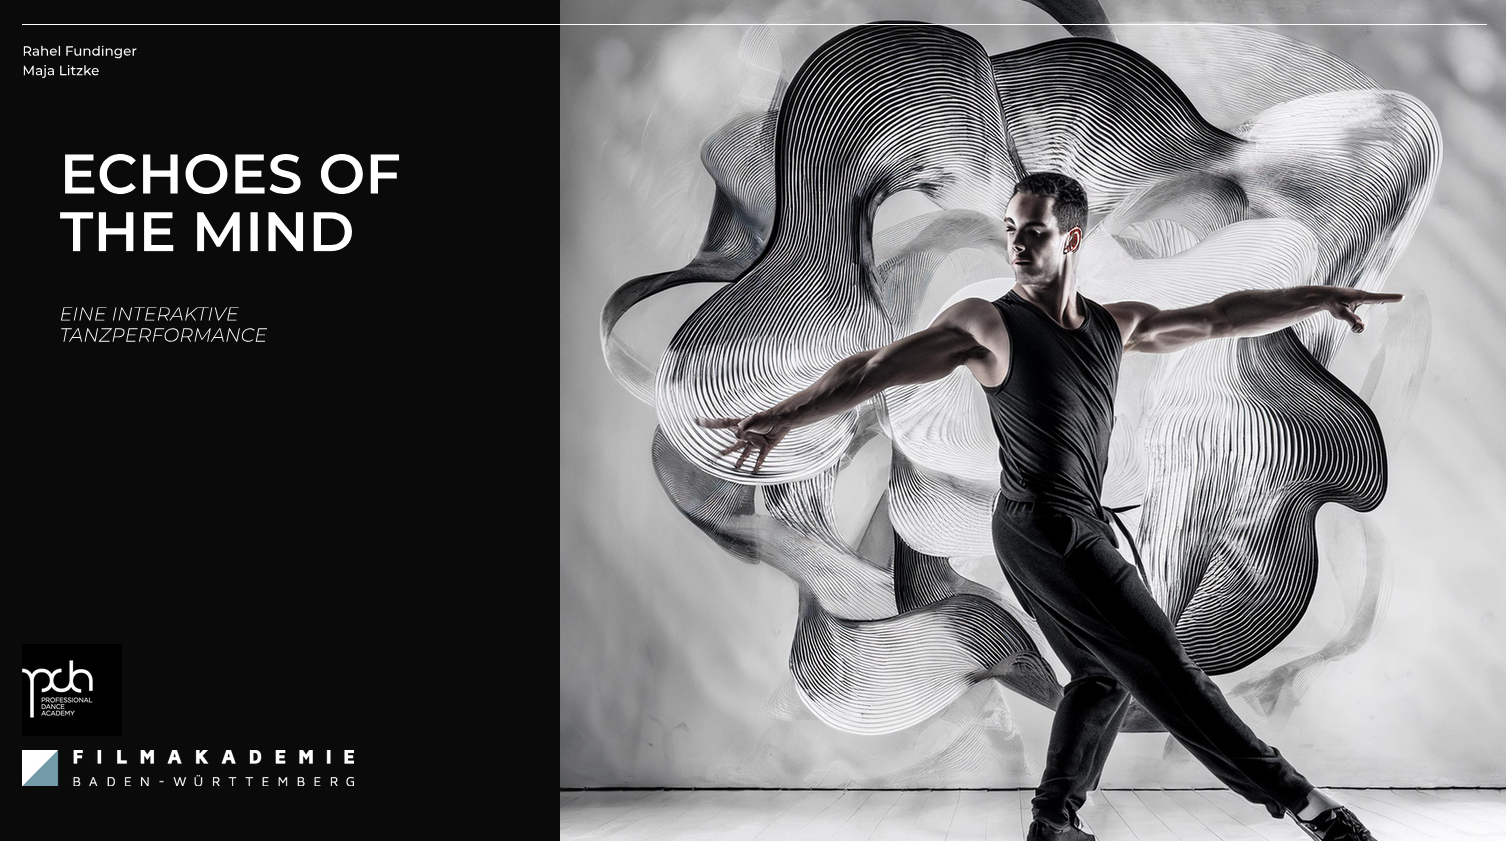
\includegraphics[width=\textwidth]{images/EchoesOfTheMind_startbild.png}
    \caption{MoodBoard-Startbild des Projektes \glqq Echoes of the Mind\grqq{}}
    \label{fig:echoes_startbild}
\end{figure}

\begin{figure}[h]
    \centering
    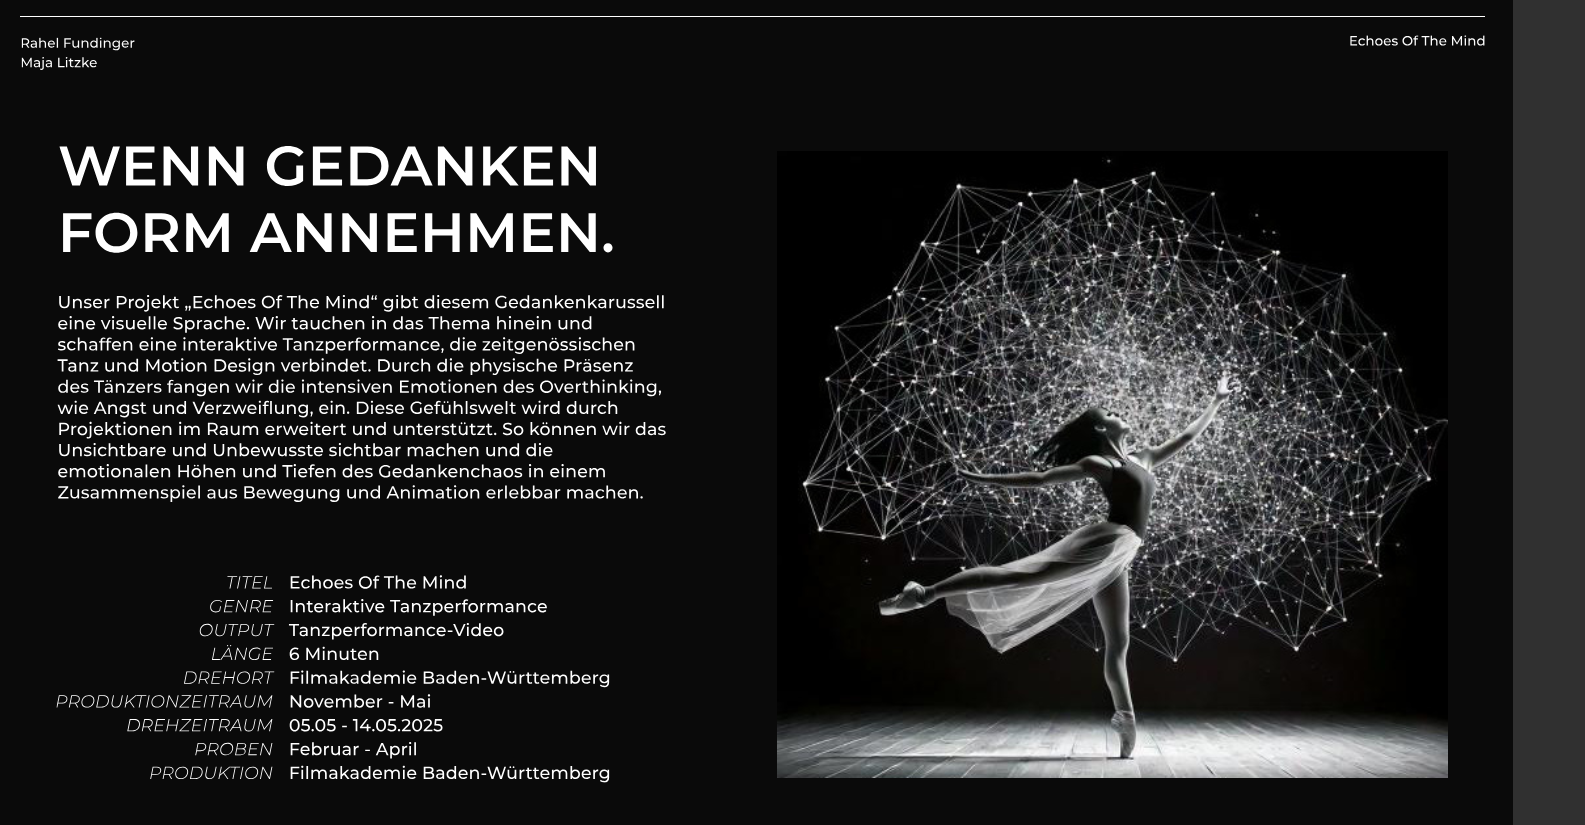
\includegraphics[width=0.9\textwidth]{images/EchoesOfTheMind_mood.png}
    \caption{Künstlerische Vision: Emotionale Visualisierungskonzepte für \glqq Echoes of the Mind\grqq{}}
    \label{fig:echoes_mood}
\end{figure}

\newpage

\textbf{Künstlerische Vision:}

Das Projekt visualisiert innere emotionale Prozesse durch externe Projektionen, die direkt auf die Körperbewegungen des Performers reagieren. Die Choreographie thematisiert mentale Überlastung und Angstzustände, wobei die technischen Visualisierungen diese psychischen Zustände räumlich und zeitlich erfahrbar machen.

\subsection{Technische Anforderungsanalyse}

Der beschriebene Projektkontext definiert spezifische technische Anforderungen für das Motion-Capture-System: variable Beleuchtungsbedingungen durch Beamer-Projektionen, schnelle und komplexe Bewegungssequenzen sowie potenzielle Teilverdeckungen des Performers während der Choreographie. 

\textbf{Spezifische Herausforderungen des Projekts:}

\begin{itemize}
    \item \textbf{Echtzeit-Responsivität:} Visualisierungen müssen unmittelbar auf Bewegungsänderungen reagieren, ohne wahrnehmbare Verzögerung
    \item \textbf{Präzise Körper-Mapping:} Projektionen sollen exakt auf spezifische Körperregionen (Kopf, Hände, Torso) ausgerichtet werden: Auch bei \textbf{Partieller Sichtbarkeit:} Tänzer verdecken oft Körperteile - Standard-Kinect verliert dann das Skelett
    \item \textbf{Beleuchtungskompatibilität:} Das System muss unter intensiver Beamer-Beleuchtung funktionieren, sowie unter geringer Lichtverfügbarkeit.
    \item \textbf{Multiple Kamerawinkel:} Verschiedene Szenen erfordern Top-Down-, Front- und Seitenperspektiven
    \item \textbf{Schnelle Setup-Wechsel:} Mehrere Visualisierungsmodi müssen innerhalb der Produktionszeit umschaltbar sein
\end{itemize}

\textbf{Produktionskontext:}

Die Filmproduktion war für Mai 2025 im professionellen Albrecht-Ade-Studio der Filmakademie Ludwigsburg geplant. Dies definierte einen festen Zeitrahmen von vier Monaten für Entwicklung, Testing und Produktionsreife des M.A.S.K.-Systems.

\newpage

\subsection{Professionelle Arbeitsteilung}

\textbf{Kreative Führung - Filmakademie Ludwigsburg:}
\begin{itemize}
    \item \textbf{Maja Litzke \& Rahel Fundinger:} Künstlerische Vision und Choreographie-Entwicklung
    \item \textbf{Produktionsinfrastruktur:} Bereitstellung von professionellem Studio, Beamer-Equipment und Kamera-Hardware
    \item \textbf{Visual Design:} Definition ästhetischer Anforderungen und emotionaler Zielstellungen
    \item \textbf{Workflow-Integration:} Einbindung in bestehende TouchDesigner-Produktionspipelines
\end{itemize}

\textbf{Technische Vollverantwortung - Hochschule Reutlingen:}
\begin{itemize}
    \item \textbf{Marty Lauterbach (Solo-Developer):} Eigenständige Entwicklung der kompletten Motion-Capture-Pipeline
    \item \textbf{System-Architektur:} Design und Implementation der MediaPipe-TouchDesigner-Integration
    \item \textbf{Entwicklung:} Infrarot-basierte Tracking-Lösung unter Produktionsbedingungen
    \item \textbf{Performance-Engineering:} Optimierung für Real-time-Anforderungen und Produktionsumgebung
\end{itemize}

\subsection{Kooperationsmanagement}

Da sich bei diesem Projekt zwei Hochschulen zu einem interdisziplinären Team zusammenfanden, wurde gemeinsam ein agiler Entwicklungsansatz gewählt. In regelmäßigen Sprint-Meetings definierten die Filmakademie-Partner die künstlerischen und choreographischen Anforderungen, während ich die technischen Möglichkeiten und Limitierungen kommunizierte. Diese bidirektionale Abstimmung ermöglichte sowohl technische Optimierungen als auch kreative Anpassungen basierend auf den jeweiligen Fachkompetenzen.

\textbf{Kommunikationsstruktur:}

Regelmäßige Online-Kommunikation ermöglichte kontinuierliche Abstimmung zwischen den Standorten Reutlingen und Ludwigsburg. Zusätzlich fanden vier Online-Meetings statt, um komplexe technische und künstlerische Entscheidungen gemeinsam zu treffen.

\textbf{Iterative Anforderungsentwicklung:}

Die Anforderungen entwickelten sich iterativ basierend auf choreographischen Erkenntnissen und technischen Möglichkeiten. Dies erforderte flexible Systemarchitektur und agile Entwicklungsmethoden, um auf Änderungen reagieren zu können.

\subsection{M.A.S.K. als technisches Backbone}

M.A.S.K. wurde als technisches Backbone entwickelt, um die künstlerische Vision zu realisieren. Das System musste spezifische Voraussetzungen erfüllen, damit die kreativen Visualisierungen den gewünschten künstlerischen Effekt erzielen können. Durch präzises Skelett-Tracking mittels Kinect V2 und MediaPipe reagieren die projizierten Visualisierungen in Echtzeit auf Bewegungen, Position und emotionale Ausdruckskraft des Performers.

\textbf{Systemintegration:}

Das entwickelte System musste sich gut in bestehende TouchDesigner-Workflows der Filmakademie integrieren, ohne bestehende Produktionsprozesse zu unterbrechen. Dies erforderte modulare Architektur und standardisierte Schnittstellen.

\textbf{Evaluierungsmetriken:}

Der Projekterfolg wurde anhand folgender Kriterien gemessen:
\begin{itemize}
    \item Zuverlässige Tracking-Performance während der gesamten Produktionszeit
    \item Kurze Setup-Zeiten pro Visualisierungsmodus
    \item Nahtlose Integration in den Filmproduktions-Workflow
    \item Künstlerische Zufriedenheit mit der Responsivität der Visualisierungen
\end{itemize}